\documentclass{article}%
\usepackage[T1]{fontenc}%
\usepackage[utf8]{inputenc}%
\usepackage{lmodern}%
\usepackage{textcomp}%
\usepackage{lastpage}%
\usepackage{authblk}%
\usepackage{graphicx}%
%
\title{Time{-}dependent onset of Interferon{-}a2b{-}induced apoptosis in isolated hepatocytes from preneoplastic rat livers}%
\author{Toni Sullivan}%
\affil{Department of Surgery, University of Wisconsin Hospital and Clinics, Madison, Wisconsin, United States of America}%
\date{01{-}01{-}2013}%
%
\begin{document}%
\normalsize%
\maketitle%
\section{Abstract}%
\label{sec:Abstract}%
The Myc retinas have an innate ability to detect small patches of (reactive) macrophage called oligobullets that could potentially allow bacteria and fungal infections to travel up the optic nerve.\newline%
Earlier this year a study from the University of Sydney (UniSM) and the University of Melbourne revealed that, by blocking an important pro{-}inflammatory receptor found on macrophages, macrophages can decrease levels of inflammatory responses that cause inflammation.\newline%
In the present study, researchers infected mice with the mutation, Myc, and exposed them to bacteria and fungal spores at two different times: two hours before infection, and eight hours after infection. Mice exposed to infection at the two times were more susceptible to the disease than mice exposed at normal incubation.\newline%
The researchers found that macrophages present in the eyes of mice and whose normal MSC proteins do not bind to Myc, are unable to fight off infection in mice exposed to infections at the eight hour incubation stage. They were able to reduce their expression of Myc and decrease the levels of inflammation.\newline%
The researchers believe that their treatment will not only decrease levels of inflammation, but also decrease immune suppression during infection, or can inhibit it during disease progression.\newline%
The treatment, being developed by the Department of Pathology at the University of Melbourne, is an experimental form of therapeutic that integrates the two hematopoietic pro{-}inflammatory modulators (MPMs), Prokopiotis Phase II and AMPK within a single therapy.\newline%
Professor Hawkedrys said: Finding drugs that can activate both two pro{-}inflammatory receptors, Prokopiotis Phase II and AMPK, is a very important and sought after technique for T{-}cell transplantation, and we hope to be able to deliver Prokopiotis Phase II/AMPK modulators in parallel with the FDA approved dose of Chronic Phase I.\newline%
On being infected with the Myc suppressor, myloid mucosa, or topline immunosuppressant IM, the mice had an immune response which decreased the levels of Myc, but these decreased only during infection and did not suppress the immune response in the days after infection.\newline%
Professor Hawkedrys said: Myc suppression was shown to be triggered early during infection. That, to me, means that the immune response can be maintained through the presence of Myc.\newline%
Journal citation\newline%
Agrieved {-} (2013) Neurone binding in macrophages, myc and immunocompromodulation pro{-}inflammatory signalling, Anti{-}Psyrimidicykinin III (Pandemic Helicobacterial Deficiency) and adaptive Elicitor Interoperation. Ibn al{-}Sudl Al{-}Ajroushi et al, doi: 10.1016/j.haazel.2012.01.005.\newline%
Conflict of Interest

%
\subsection{Image Analysis}%
\label{subsec:ImageAnalysis}%


\begin{figure}[h!]%
\centering%
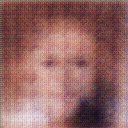
\includegraphics[width=150px]{500_fake_images/samples_5_327.png}%
\caption{A Man With A Beard Wearing A Tie And Glasses}%
\end{figure}

%
\end{document}